\documentclass[aspectratio=169]{beamer}
\usepackage{color,amsmath}
\usepackage{subfigure}
\usepackage{booktabs}
\usepackage{framed}
\usepackage{comment}

\def\vf{\vfill}

%%%%%%%%%%%%%%%%%%%%%%%%%%
\title[]{Making it happen}
\author[]{Matthew J. Salganik\\Department of Sociology\\Princeton University}
\date[]{Summer Institute in Computational Social Science\\June 24, 2017
\vfill
\begin{flushright}
\vspace{0.6in}

\includegraphics[width=0.1\textwidth]{figures/cc-by.png}
\end{flushright}
}
\begin{document}
%%%%%%%%%%%%%%%%%%%%%%%%%%
\frame{\titlepage}
%%%%%%%%%%%%%%%%%%%%%%%%%%
\begin{frame}

\begin{center}
\only<1>{
\includegraphics[width=\textwidth]{figures/exp_making_it_happen_slides_1}}
\end{center}

\end{frame}
%%%%%%%%%%%%%%%%%%%%%%%%%%
\begin{frame}

How to partner with the powerful?

\end{frame}
%%%%%%%%%%%%%%%%%%%%%%%%%%
\begin{frame}

\begin{itemize}
\item Partner, not I want them to give me their data
\pause
\item Start personal relationships
\pause
\item Do internships
\pause
\item Find Pasteur's Quadrant
\end{itemize}

\end{frame}
%%%%%%%%%%%%%%%%%%%%%%%%%%
\begin{frame}

\begin{center}
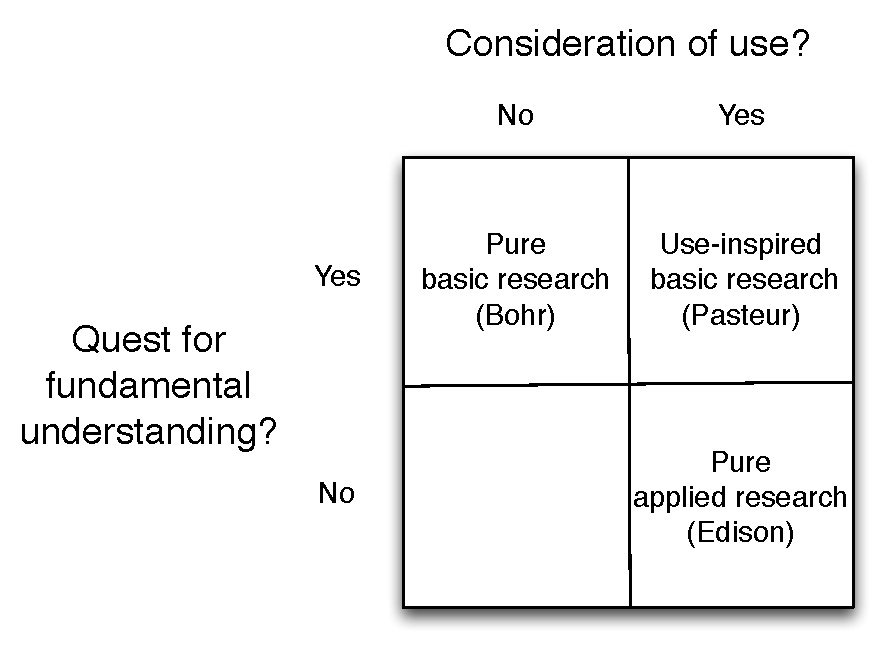
\includegraphics[width=0.6\textwidth]{figures/bitbybit4-17_pasteurs_quadrant}
\end{center}

\end{frame}
%%%%%%%%%%%%%%%%%%%%%%%%%%
\begin{frame}

\begin{center}
\only<1>{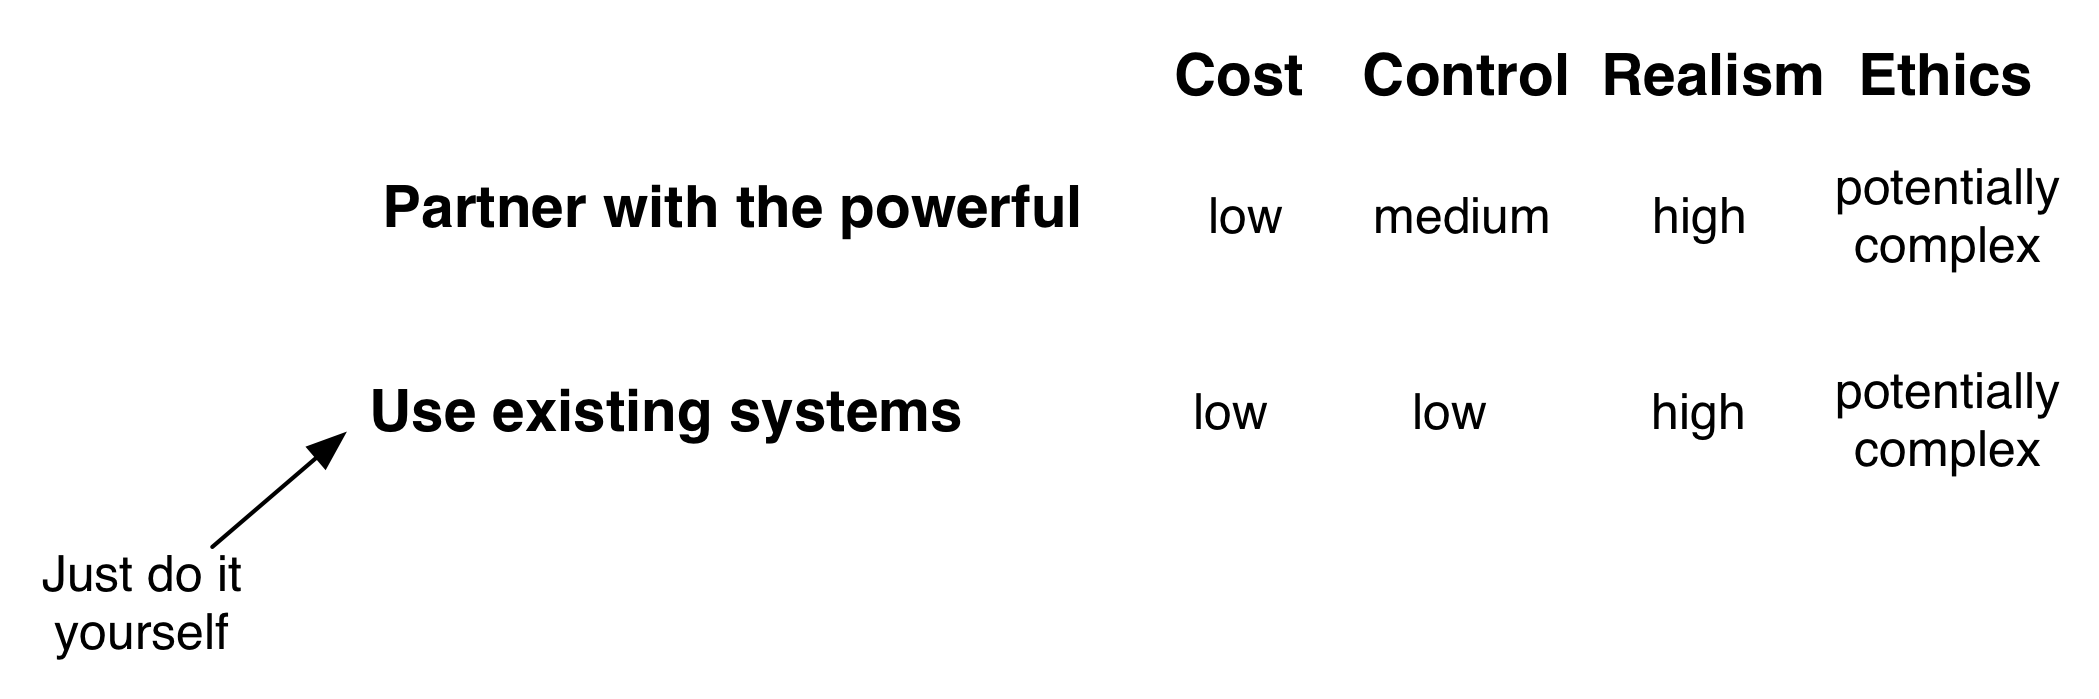
\includegraphics[width=\textwidth]{figures/exp_making_it_happen_slides_2}}
\only<2>{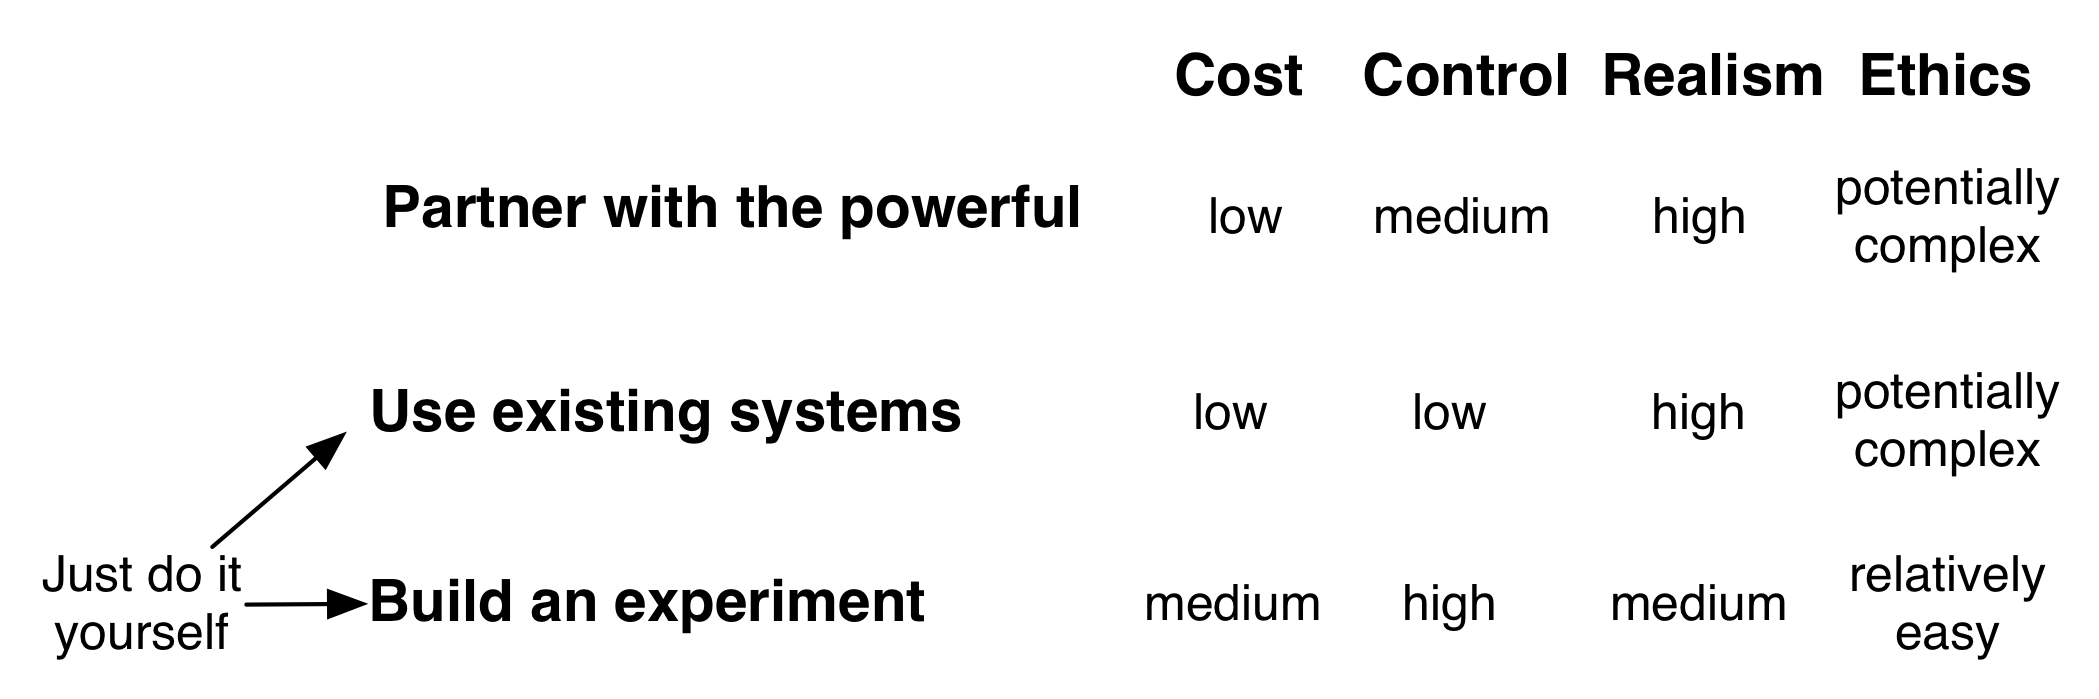
\includegraphics[width=\textwidth]{figures/exp_making_it_happen_slides_3}}
\only<3>{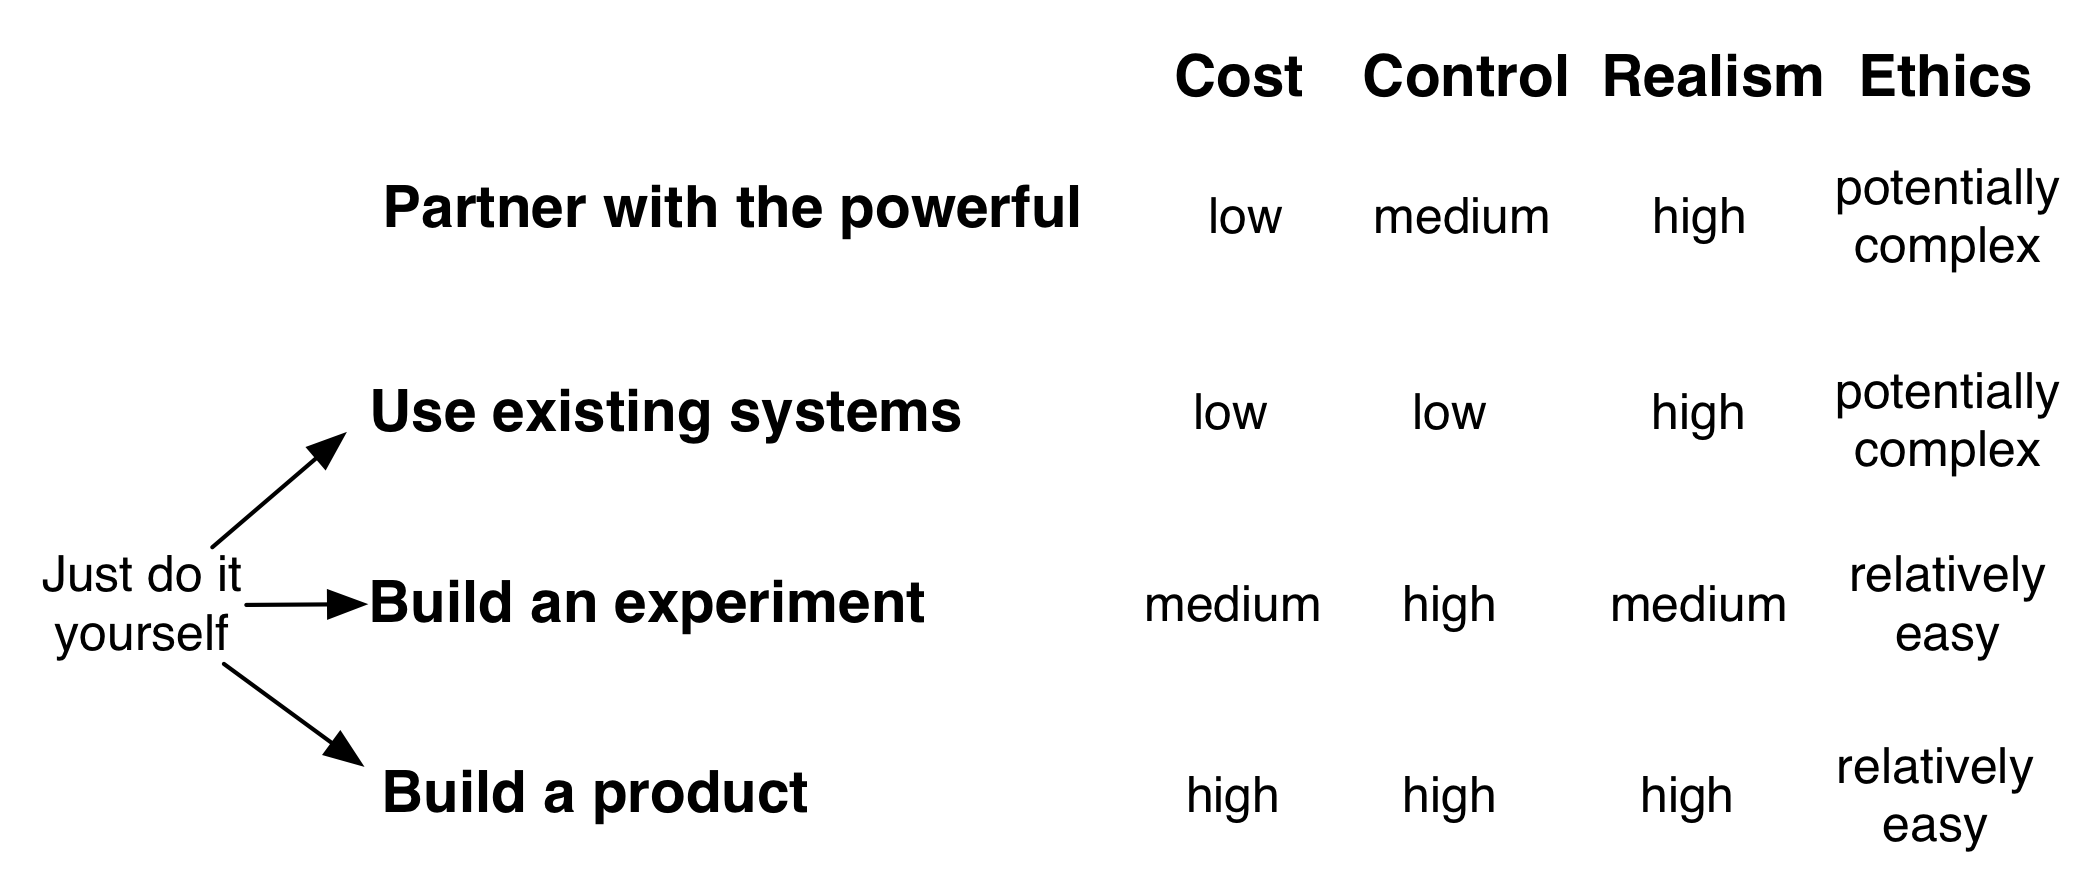
\includegraphics[width=\textwidth]{figures/exp_making_it_happen_slides_4}}
\end{center}

\end{frame}
%%%%%%%%%%%%%%%%%%%%%%%%%

\end{document}
